% Brief: approach + experimental setup + the relevant physics/maths (for a camera: the measurement
% model). System overview first, then subsystems.
\section{Method}
\label{sec:method}

\begin{figure}[t]
  \centering
  \placeholder{System photo with labels: monitor, fan with letter cards, matte black backing,
  camera, Raspberry Pi, Arduino + stepper driver. Inset: block diagram of signals and timing.}
  \caption{\TODO{The rig. Say what each part does and how far the camera is from the fan.}}
  \label{fig:system}
\end{figure}

\subsection{System overview}
\label{sec:overview}
The rig has three parts (\cref{fig:system}). An Arduino Uno drives a 28BYJ-48 stepper motor through a
ULN2003 driver, spinning a fan whose blades carry printed letters in front of a matte black backing.
A Raspberry Pi runs the camera and, on its own monitor facing the fan, shows a black/white code with
one bit per four \SI{60}{Hz} refreshes. One button in our capture software starts one long exposure
and the code together and saves the raw image with a log of when each bit was shown. Reconstruction
runs offline on a laptop. \TODO{Fan dimensions and camera distance.}

\subsection{Measurement model}
\label{sec:model}
After unwrapping the image to polar coordinates $(r,\theta)$ about the hub, a rotation at angular
speed $\omega$ is a shift along $\theta$. We discretise the exposure into short time steps $t_k$ of
length $\Delta t$. A polar sample $i$ on sensor line $\ell_i$ then records
\begin{equation}
  b_i = \sum_k w_k(\ell_i)\, x(\theta_i - \omega t_k) + n_i,
  \label{eq:forward}
\end{equation}
\begin{equation}
  w_k(\ell) = L(t_k)\,\bigl|[t_k - \tfrac{\Delta t}{2}, t_k + \tfrac{\Delta t}{2}) \cap [s_\ell, s_\ell + T)\bigr|,
  \label{eq:weights}
\end{equation}
where $x$ is the sharp image, $L(t)\in\{0,1\}$ the monitor brightness, $T$ the exposure, $s_\ell$ the
time line $\ell$ opens, and $n_i$ noise. Equation~\eqref{eq:forward} is linear in $x$, and with linear
interpolation in $\theta$ each ring of radius $r$ gives a sparse matrix,
$\mathbf{b}_r = \mathbf{A}_r(\omega)\,\mathbf{x}_r + \mathbf{n}_r$. Because the arc in view does not
wrap around, $\mathbf{x}_r$ extends beyond the window to hold light that moves into it during the
exposure.

The code decides whether $\mathbf{A}_r$ can be inverted. Under steady light the blur is a box whose
spectrum has exact zeros; a good code keeps every frequency well above zero (\cref{fig:code}).

\subsection{Global and rolling shutter}
\label{sec:shutters}

\begin{figure}[t]
  \centering
  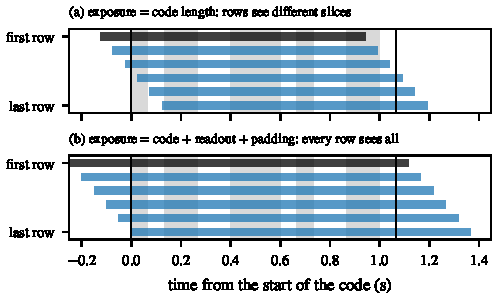
\includegraphics[width=\linewidth]{timing}
  \caption{When each sensor row collects light (bars) relative to the code (grey: monitor on), drawn
  for six rows with the readout four times longer than the rolling shutter camera's
  \SI{64}{ms} so that the stagger is visible. (a) With the exposure equal to the code, each row sees
  a different slice of the code, so one blur for the whole frame is wrong for most rows. (b) Our
  capture software lengthens the exposure by the readout time plus \SI{50}{ms}, so every row sees
  the whole code.}
  \label{fig:timing}
\end{figure}

The three methods differ only in $s_\ell$ in \eqref{eq:weights}. A global shutter opens every line
at once ($s_\ell = 0$). A rolling shutter opens line $\ell$ of $H$ at $s_\ell = \ell\,T_\mathrm{ro}/H$,
where $T_\mathrm{ro}$ is the readout time. \emph{Per row} uses each sample's own $s_\ell$;
\emph{per frame} uses the middle line's $s_\ell$ for every sample, as a pipeline that ignores the
rolling shutter would. \Cref{fig:timing}a shows why per frame then fails: the rows see different
slices of the code. Our capture software avoids this by construction (\cref{fig:timing}b): it
exposes for the code plus the readout plus \SI{50}{ms} of padding, so every row sees the full code
and the two rolling shutter methods coincide. We therefore compare them in simulation with the
exposure equal to the code, where they differ most.

\subsection{Reconstruction}
\label{sec:recon}
The baseline solves each ring by Tikhonov-regularised least squares with a first-difference
penalty $\mathbf{D}$,
\begin{equation}
  \hat{\mathbf{x}}_r = \arg\min_{\mathbf{x}} \|\mathbf{A}_r\mathbf{x}-\mathbf{b}_r\|_2^2
  + \lambda\|\mathbf{D}\mathbf{x}\|_2^2 .
  \label{eq:tikhonov}
\end{equation}
The main solver is DPIR~\cite{zhang2022plug}: half-quadratic splitting that alternates a data step
with a pretrained denoising network (DRUNet) acting as the prior, applied to all rings at once
through the block-diagonal operator. It needs no tuning. We scale the operator to unit gain and set
the noise level to six times a wavelet estimate from the polar data; the estimate reads about a
third of the true noise after resampling, and DPIR performed best at twice the true noise.

\subsection{Speed from a single photograph}
\label{sec:speed}
A wrong speed predicts the wrong blur, which DPIR cannot fit without breaking its prior. We therefore
reconstruct a band of 64 rings at 21 candidate speeds spanning $\pm20\%$ of the commanded speed, take
the data residual $\|\mathbf{A}(\omega)\hat{\mathbf{x}}(\omega)-\mathbf{b}\|_2$ at each, and refine the
minimum with a parabola through its neighbours. The same residual checks the direction of rotation:
if $-\omega$ fits better than $+\omega$ by a margin of 10\%, the sign is flipped.

\subsection{Calibration}
\label{sec:calibration}
The pipeline needs the hub centre, the radii of the blades and the arc they occupy. We find all
three from three photographs of the stopped fan, turned by a known number of motor steps between
them (\SI{4076}{} half-steps per revolution). For each pair of photographs we search for the centre
about which one rotates into the other, first on a coarse grid and then by Nelder-Mead; the median
over the pairs is the hub, and a spread above \SI{1}{px} warns that the camera moved. The code timing
comes from each capture's log, and a photograph of the stopped fan in the same setup is the
reference for image quality. \TODO{Measured hub spread on the rig: \X~px.}

\subsection{Experimental protocol}
\label{sec:protocol}

\begin{table}[t]
  \centering\small
  \caption{Rig and capture parameters. Readout times are the capture software's estimate (one over
  the sensor mode's maximum frame rate), logged with every capture. \TODO{Update the code if it is
  replaced (\cref{sec:limitations}).}}
  \label{tab:params}
  \begin{tabular}{@{}ll@{}}
    \toprule
    Parameter & Value \\
    \midrule
    Code & \rigBits~bits, \rigCodeMs~ms each, \rigCodeS~s \\
    Exposure & code + readout + \SI{0.05}{s} \\
    Global shutter camera & Sony IMX296, $1456\times1088$ \\
    Rolling shutter camera & OV5647, $2592\times1944$ \\
    Readout, global / rolling & 16.6 / \SI{64.0}{ms} \\
    Motor & 28BYJ-48, \SI{4076}{} half-steps/rev \\
    Fan speeds & \TODO{3, 5, 8, 10}~rpm \\
    Captures per condition & 10 \\
    Camera to fan & \X~cm \\
    \bottomrule
  \end{tabular}
\end{table}

\paragraph{Simulation.} Before the rig existed we validated the pipeline on renders. Blender renders
a single \SI{50}{mm} blade filling the frame height, hub above the frame, on a black background, at
$728\times544$~px in steps of \SI{8.3}{ms} while it turns at \SI{0.35}{rpm}; one scene carries
letters, a harder one a photograph plus letters. We apply the code and each line's exposure window
in software, then a sensor model with Poisson shot noise, a \SI{10000}{e^-} full well, \SI{3}{e^-}
read noise and a 10-bit converter, with steady light filling 70\% of the well on white. The code is
the 52-bit code of~\cite{raskar2006coded} at one bit per refresh (\SI{0.87}{s}). The short exposure
baseline is a single \SI{16.7}{ms} bit with $16\times$ analogue gain.

\paragraph{Rig.} \TODO{For each speed (\cref{tab:params}): 10 coded captures, 10 with steady light,
10 short exposures, and a reference photograph of the stopped fan in the same setup. Ground truth
speed from the step rate. Dark room.}
